\chapter{Inleiding}

\section{Doel van deze handleiding}

Deze handleiding voor Trello is uitgewerkt met het oog op het gebruik tijdens de opleidingsonderdelen Projecten II en Projecten III. Dit document is zowel uitgeschreven voor programmeurs als systeembeheerders. Als een bepaald onderdeel voor slechts een van de twee groepen bedoeld is dan zal dit duidelijk aangegeven worden.

\section{Wat is Trello}

Trello\footnote{\url{http://www.trello.com}} is een gratis platform dat toelaat om in groep aan een project te werken volgens de Agile methode. Om dit te realiseren kunnen er in Trello borden aangemaakt worden waarop de groepsleden taken kunnen beheren. Dit laat de groep toe om een overzicht te krijgen van het uitgevoerde werk, op elk moment, tijdens de huidige iteratie. Daarnaast biedt het ook de mogelijkheid om na afloop van elke iteratie van het project zogenaamde ``burn-down charts'' te genereren om zo te kunnen reflecteren en bij te sturen naar een volgende iteratie toe.

\section{Benodigdheden}

Om Trello te kunnen gebruiken dien je een account aan te maken door middel van een registratie op de website \url{www.trello.com}. Gebruik bij registratie jouw Hogent e-mailadres zodat je medestudenten later gemakkelijk aan jouw team of bord kan toevoegen.\\

\noindent
\\Daarnaast dien je ook de invoegtoepassing ``Plus For Trello''\footnote{\url{http://www.plusfortrello.com}} te installeren. Deze werkt \textbf{ENKEL} met Google Chrome\footnote{\url{http://www.chrome.com}}. Indien de installatie succesvol was zal je vanaf nu na aanmelden het icoon \korteverwijzing[fig:plusfortrello] rechtsboven zien verschijnen. De eerste maal dat je aanmeldt na installatie van de invoegtoepassing kan je het best de tour volgen om zo al een inleiding te krijgen in de mogelijkheiden met ``Plus for Trello''.

\begin{figure}[h]
	\centering
	
\includegraphics[scale=.8]{./afbeeldingen/plusfortrello.png}
	\caption{Icoon ``Plus For Trello'' na installatie}
	\label{fig:plusfortrello}
\end{figure} 
\noindent
\textbf{AANDACHT:} Voer zeker volgende configuratie uit in ``Trello for Plus''. 
\paragraaf{Synchronisatie}
\noindent
\\Stel de synchronisatie correct in om te vermijden dat teamleden en begeleidende lector(en) andere tijdsmetingen waarnemen dan jij zelf. Om er voor te zorgen dat iedereen dezelfde uren zal zien stel je de synchronisatie in als volgt:
\begin{enumerate}[nolistsep]
	\item Klik op het zandloper icoontje van ``Plus for trello'' \korteverwijzing[fig:plusfortrello]
	\item Klik onder ``contents'' op ``Sync (by Card comment keywords or Stealth)''
	\item Verander, indien nodig, de waarde in de lijst naar ``Recommended -Store inside Trello (S/E in Trello card comments)'' \korteverwijzing[fig:synctrello]
\end{enumerate}

\begin{figure}[h]
	\centering
	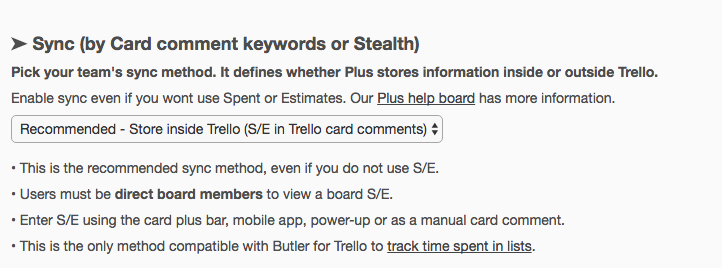
\includegraphics[width=\textwidth]{./afbeeldingen/synctrello.png}
	\caption{Instellen synchronisatie tijden in ``Plus For Trello''}
	\label{fig:synctrello}
\end{figure} 
\pagebreak
\paragraaf{Negatieve waarden voor R toelaten}
\noindent
\\Hoeveel tijd je nodig hebt om een taak af te ronden is niet makkelijk in te schatten.  Het kan dus gebeuren dat de geschatte tijd (E) lager ligt dan de effectief gepresteerde tijd (S). Hierdoor zal het aantal overgebleven uren (R) voor een kaart negatief uitvallen. Indien de optie in ``Plus For Trello'' niet geactiveerd is om negatieve uren toe te laten, zal automatisch het aantal E uren verhoogd worden als het aantal S uren boven die waarde  gaat. Hierdoor zal het aantal R uren nooit onder 0 komen te liggen. Dit is uiteraard geen juiste weergave van de verrichte prestaties, activeer daarom deze optie als volgt:
\begin{enumerate}[nolistsep]
	\item Klik op het zandloper icoontje van ``Plus for trello'' \korteverwijzing[fig:plusfortrello];
	\item Klik onder ``contents'' op ``Preferences'' en voer volgende instellingen uit \korteverwijzing[fig:prefsplusfortrello]
	\begin{itemize}
		\item Selecteer bij ``Work units'' de waarde ``hours'' indien nodig;
		\item Selecteer bij ``Week starts'' de waarde ``Monday'' indien nodig;
		\item Vink het vakje voor ``Allow negative Remaining (or never use Estimates).'' aan.
	\end{itemize}
\end{enumerate}

\begin{figure}[h]
	\centering
	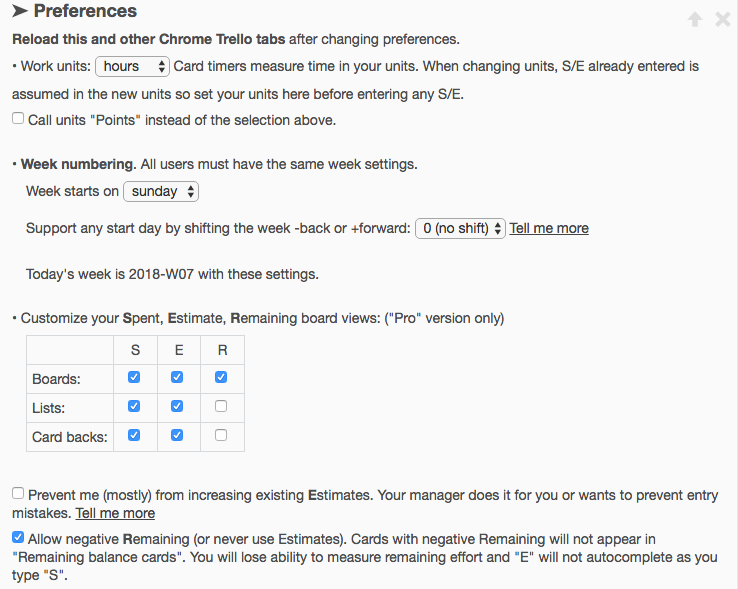
\includegraphics[width=\textwidth]{./afbeeldingen/prefsplusfortrello.png}
	\caption{Voorkeuren in ``Plus For Trello''}
	\label{fig:prefsplusfortrello}
\end{figure} 

\section{Overzicht}

Nadat je de invoegtoepassing heeft ge\"installeerd en bent aangemeld op de website krijg je een overzichtsscherm te zien met al jouw persoonlijke borden \korteverwijzing[fig:overzicht].

\begin{figure}[!h]
	\centering
	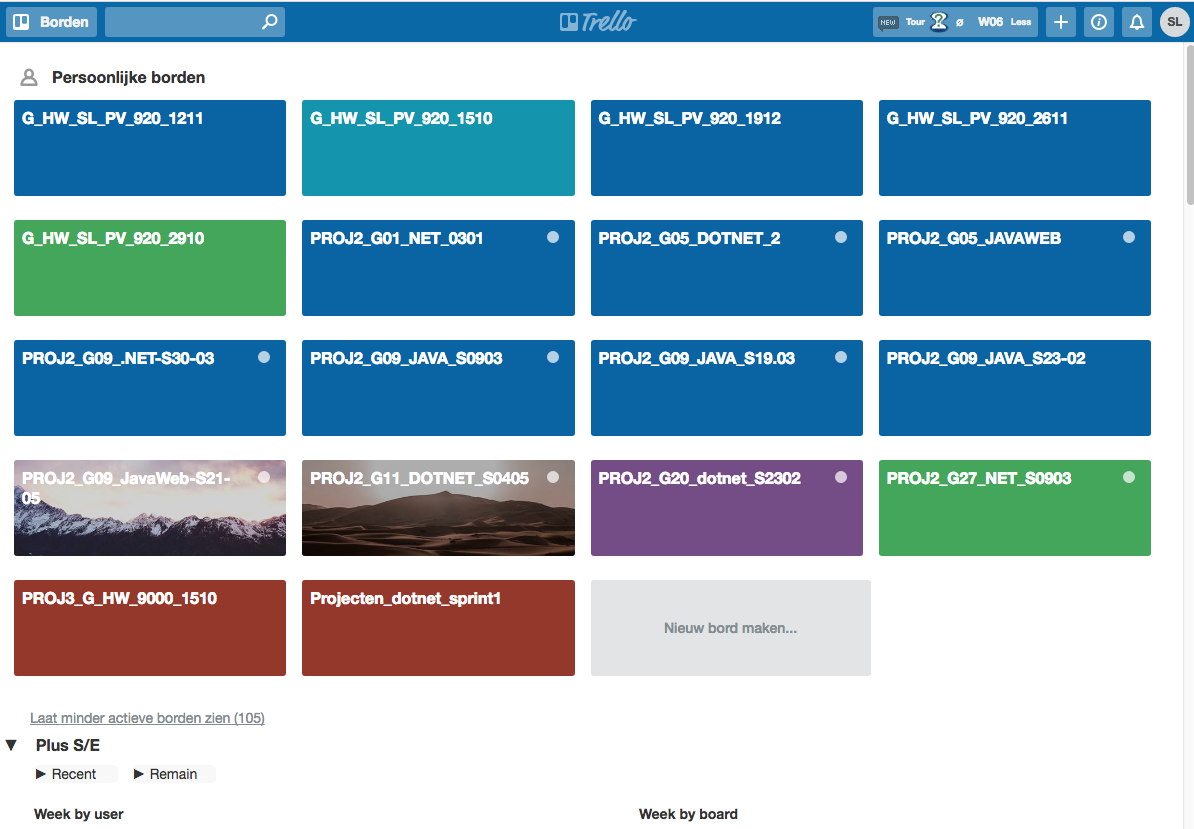
\includegraphics[width=\textwidth]{./afbeeldingen/overzicht.png}
	\caption{Hoofdscherm Trello}
	\label{fig:overzicht}	
\end{figure} 

\noindent
\\\\Volgende lijst toont een overzicht met functionaliteiten die overeenstemt met een nummer op figuur \ref{fig:overzicht_genummerd}. De belangrijkste functionaltieiten worden uitgebreid beschreven in deze handleiding.\\
\begin{enumerate}[nolistsep]
	\item Lijst borden
	\item Zoekfunctie
	\item Plus for Trello
	\item Aanmaken (Bord, team, bedrijfsteam) 
	\item Informatie
	\item Meldingen
	\item Account beheren
	\item Persoonlijke borden
	\item Nieuw bord maken
\end{enumerate}

\begin{figure}[!h]
	\centering
	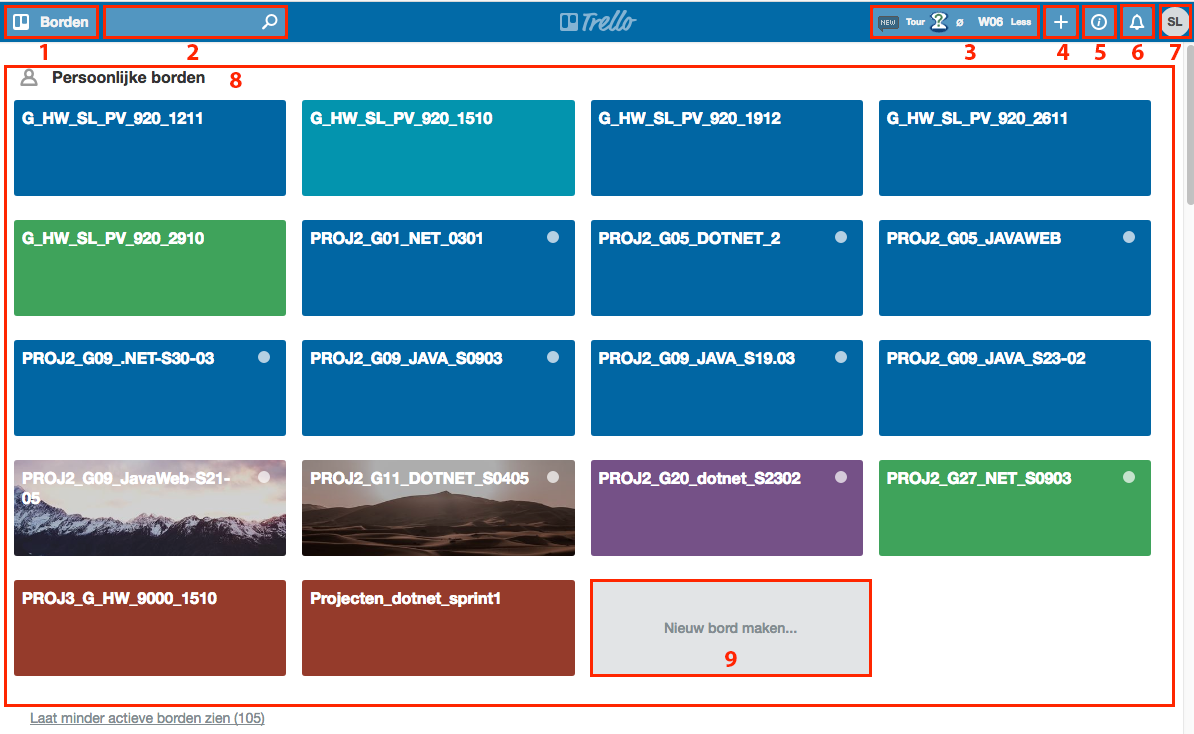
\includegraphics[width=\textwidth]{./afbeeldingen/overzicht_genummerd.png}
	\caption{Hoofdscherm Trello met aangeduide functionaliteit}
	\label{fig:overzicht_genummerd}	
\end{figure} 

\section{Stappenplan (Programmeren)}

Om snel met Trello aan de slag te kunnen gaan vind je hieronder een overzicht van stappen die voor elk project (Programmeren) moeten uitgevoerd worden in deze chronologische volgorde:
\begin{enumerate}[nolistsep]
	\item Maak jouw team aan voor het project dat bestaat uit jezelf en je groepsgenoten (Dit moet slechts door \'e\'en iemand gebeuren);
	\item Maak een nieuw bord aan met gewenste naamgeving voor jouw team;
	\item Voeg de betrokken lector(en) als lid (= Beheerder) toe aan jouw bord;
	\item Voeg lijsten toe op het bord (``Product backlog'', ``Sprint backlog'', ...);
	\item Voeg kaarten toe aan de lijst ``Product backlog'' OF kopieer de resterende kaarten uit deze lijst van een vorige sprint (bord);
	\item Verplaats de kaarten voor de huidige sprint naar ``Sprint backlog'' en voeg een inschatting (E uren) per teamlid toe aan elke verplaatste kaart;
	\item Voeg elke geleverde prestatie (S uren) per teamlid toe aan de bijhorende kaart;
	\item Verplaats een kaart indien zijn status wijzigt naar de bijhorende lijst;
	\item Herhaal stap 7-8 tijdens de huidige sprint;
	\item Ga terug naar stap 2 voor de volgende sprint.
\end{enumerate}

\section{Stappenplan (Systeembeheer)}

Om snel met Trello aan de slag te kunnen gaan vind je hieronder een overzicht van stappen die voor elk project (Systeembeheer) moeten uitgevoerd worden in deze chronologische volgorde:
\begin{enumerate}[nolistsep]
	\item Maak jouw team aan voor het project dat bestaat uit jezelf en je groepsgenoten (Dit moet slechts door \'e\'en iemand gebeuren);
	\item Maak een nieuw bord aan met gewenste naamgeving voor jouw team;
	\item Voeg de betrokken lector(en) als lid (= Beheerder) toe aan jouw bord;
	\item Voeg lijsten toe op het bord (``Backlog'', ``Ready'', ...);
	\item Voeg kaarten toe aan de lijst ``Backlog'';
	\item Verplaats een kaart van ``Backlog'' naar ``Ready'' en voeg een inschatting (E uren) per teamlid toe aan deze kaart;
	\item Voeg elke geleverde prestatie (S uren) per teamlid toe aan de bijhorende kaart;
	\item Verplaats een kaart indien zijn status wijzigt naar de bijhorende lijst;
	\item Herhaal stap 6-8 (ook 5 indien nodig) zolang het project loopt.
\end{enumerate}